\documentclass{article}

% if you need to pass options to natbib, use, e.g.:
%     \PassOptionsToPackage{numbers, compress}{natbib}
% before loading neurips_2019

% ready for submission
% \usepackage{neurips_2019}

% to compile a preprint version, e.g., for submission to arXiv, add add the
% [preprint] option:
%     \usepackage[preprint]{neurips_2019}

% to compile a camera-ready version, add the [final] option, e.g.:
     \usepackage[final]{neurips_2019}

% to avoid loading the natbib package, add option nonatbib:
%     \usepackage[nonatbib]{neurips_2019}

\usepackage[utf8]{inputenc} % allow utf-8 input
\usepackage[T1]{fontenc}    % use 8-bit T1 fonts
\usepackage{hyperref}       % hyperlinks
\usepackage{url}            % simple URL typesetting
\usepackage{booktabs}       % professional-quality tables
\usepackage{amsfonts}       % blackboard math symbols
\usepackage{nicefrac}       % compact symbols for 1/2, etc.
\usepackage{microtype}      % microtypography
\usepackage{graphicx}
\usepackage{float}


\graphicspath{{./graphics/}}
\title{Twitter sentiment analysis using LSTM}

% The \author macro works with any number of authors. There are two commands
% used to separate the names and addresses of multiple authors: \And and \AND.
%
% Using \And between authors leaves it to LaTeX to determine where to break the
% lines. Using \AND forces a line break at that point. So, if LaTeX puts 3 of 4
% authors names on the first line, and the last on the second line, try using
% \AND instead of \And before the third author name.

\author{%
  Adam Lewandowski, Ivan Sladkov, Patrick Cormac English  \\
  School of Computer Science\\
  University College Dublin\\
  Belfield, Dublin 4, Ireland \\
  \texttt{adam.lewandowski@ucdconnect.ie} \\
  \texttt{ivan.sladkov@ucdconnect.ie} \\
  \texttt{patrick.english@ucdconnect.ie} \\
  % examples of more authors
  % \And
  % Coauthor \\
  % Affiliation \\
  % Address \\
  % \texttt{email} \\
  % \AND
  % Coauthor \\
  % Affiliation \\
  % Address \\
  % \texttt{email} \\
  % \And
  % Coauthor \\
  % Affiliation \\
  % Address \\
  % \texttt{email} \\
  % \And
  % Coauthor \\
  % Affiliation \\
  % Address \\
  % \texttt{email} \\
}

\begin{document}

\maketitle

\begin{abstract}
  In the advent of social media, forums, blogs, product review pages and other
  streams of human generated e-content, internet has become the de facto
  standard for human interactions and outlet for their opinions and emotions.
  This makes it a perfect resource for sentiment analysis, which can serve as
  critical information in the decision making process for businesses and
  politicians alike[1]. In this report we are especially focusing on tweet
  sentiment analysis. We discuss challenges and findings associated with it, as
  well as compare performance of modern LSTMarchitecture with old state of the
  art. Moreover, we discuss necessary text pre-processing techniques and
  describe the whole process of LSTM model construction.
\end{abstract}

\section{Introduction}

As micro-blogging websites, such as Facebook and Twitter, have proliferated in
both size and popularity, there has been a concomitant growth in interest in
data-extraction of the audiences and user-bases of these platforms.The data
available on these platforms is both high-volume and complex,presenting
challenges for both pre-existing and novel-model based analysis.One aspect of
this data in particular, “Sentiment”, has been the focus of extensive research
in the field of model-based analysis. Financial, commercial, and political
applications exist for the effective analysis of user-sentiment, and there has
been particular emphasis on Twitter as a “real-time” source of user sentiment in relation to events.
\par
This work will assess a variety of model-based approaches to assessing user
sentiment, in particular the performance distinctions that arise between what
might be termed “Deep Learning” approaches (Neural Networks – Recursive and
Convolutional), and a variety of non-Deep Learning approaches. A shared
pre-processing stage was developed, with a number of operations applied
uniformly to a Twitter dataset (“Tweets”) in anticipation of model training and prediction.
\par
In addition to the initial assessment, an additional generalisation test is
included as part of the experimental framework. This measures the performance of
models on a “newer” Twitter dataset (with the same pre-processing stages), to
identify model robustness across deviations in language and user tendencies.

\section{Related work}

This area has been subject to a variety of approaches using the models
identified above, and a broad survey of existing works has been carried out as a
preparatory step for this report.
\par
Initial vectorisation of tweet data was considered with respect to the work
undertaken by Hitesh et al. The need to reduce/transform input features in a
manner most conducive to the dataset was appreciated at the outset of this work,
and Word2Vec and TFIDF were both identified as viable candidates. TFIDF assigns
word scores based on document appearance, and has been identified as a useful
basis for establishing word importance, in addition broad categorisation of
documents. Word2Vec is a shallow-Neural Network approach that maps input words
to a vector space, identifying common linguistic context. A number of
considerations were identified with respect to the work by Hitesh et al. and
their choice to employ Word2Vec. Key motivating factors in their choice were a)
Dimensionality reduction and b) semantic relationship identification. In the
corpus utilised for this work, it was identified that a) tweets were short, and
shared significant vocabulary components (once pre-processing steps were
executed) and b) topic identification provided, in the authors’ view, a more
readily accessible mode of sentiment grouping than semantic contextualisation.
The two Deep-learning models employed in this study also allowed for inherent
semantic encoding, and so specific pre-processing in this regard was judged
extraneous. Further, as computational resources were limited for this survey,
TFIDF provided a more manageable process. On that basis, TFIDF was identified as
a more desirable vectorisation process, and was employed for this assessment.
\par
Further to this, a survey was conducted of viable model options for the
non-Neural Network paradigm assessment. In this regard, the above work by Hitesh
et al. was persuasive in setting out a basis for the use of Random Forest model,
albeit in that case it was paired with Word2Vec, and so deviation in performance
was anticipated. Tyagi et al. established a similar basis for the use of k-nn
classifiers. It should be noted that performance deviations were, once again,
anticipated, as that study did not make use of vectorisation and instead
employed a “bag of words” approach. A similar issue was identified with the use
of Naieve Bayes classifiers, as employed by Suppala et al. It was identified
however that those models were not incompatible with a vectorisation step, and
indeed may derive some benefits from it. Two regression-based methods were
identified as suitable for this study based on analysis of the literature:
Logistic Regression classification, as per Tyagi et al. and Support Vector
Machines, as based upon assessment of Ahmad et al.
\par
Having considered the non-Neural Network baseline models, an assessment was made
of both Recursive and Convolutional approaches, identified as desirable in Van
et al. and Severyn et al. RNNs presented several favourable characteristics for
this task, notably capture of sequential information, and shared parameters.
Given the repetitive nature, and context dependency, of the Tweet data, RNNs
were assessed as suitable for this survey. Further to this, issue with gradients
(“vanishing”) were assessed as unlikely in this context, given the brevity of
input data. CNNs were also identified as suitable, based on the assessment of
Severyn et al. The ability to capture word sequences within the vectorised data
was identified as desirable, given the dependencies inherent in certain
sentiment-sensitive terms.
\par
\section{Experimental setup}
Following steps identified in Hitesh et al. and Burns, a number of steps were
taken before vectorisation in order to maximise information density within the
input data.
\subsection{Punctuation removal}
A straightforward string check was employed to remove a variety of punctuation
symbols. Given the level at which the data will be provided to the models for
training, punctuation encodes no significant semantic information, and can be
removed without detriment to model performance.
\subsection{Stop-word removal}
Stop-words are those words which do not convey “content” in the sense of
specific references within the data, and instead represent common,
intra-sentence data such as particles (“to”), prepositions (“on”), etc. These
words were identified through the NLTK package, and replaced using the same
methodology as in step a). While it is possible for data to be encoded within
stop-words, given the aforementioned level at which data will be provided to the
models (high-level – topics, key-words), these words can be removed without
detriment to model performance.
\subsection{POS-tagging}
POS-tagging refers to identifying word roles within a sentence (noun, verb,
etc.). This is necessary where, as in part d), lemmatizing is employed for word
reduction.
\subsection{Lemmatizing}
Many words can be reduced to some simpler form (ie. “fish” from “fishing” and
“fished”). Given the relatively small dataset, it was decided to perform
lemmatizing (reduction of words to root, as above), rather than stemming.
Stemming is a simpler method, where reductions are made on the basis of
string-based rules (eg. remove all “ing” strings). This is a quick method, but
can result in illegal word truncation. Lemmatizing, the removal of morphological
affixes (the “ing”, “ed” in the example above), was chosen as providing a more
suitable base for the task.
\subsection{Vectorization}
After the application of pre-processing steps to the data, a TFIDF matrix was
developed using the scikit\_learn package (TfidfVectorizer). This implicitly
involves the following operations: creation of a term frequency matrix
(identifying the occurrence or not of a given term within a document), a
document frequency matrix (identifying the occurrence or not of a given term
across the documents), and finally an inverse document frequency (log N/O, where
N is the number of documents, and O was the number of documents in which a term
occurred). The TF-IDF score can then be obtained by obtaining the product of a
term frequency and IDF score.
\subsection{Non-NN environment setup}
gdfgdfg
\subsection{NN environment setup}
gdfgdf
\subsection{Pre-processing for deep learning models}
For the deep learning models, we decided to use the embedding layers provided by
the Keras library to generate the word vectors for every word in the dataset.
Before training the models using the data, we had to apply some extra
pre-processing. The embedding layers in Keras require arrays of integers of a
fixed size as an input, so the first thing we had to do was transform the tweets
from single strings to arrays of integers representing every word in the
sentence. The first step was creating a dictionary of the words in the dataset.
It is important to limit the words used in the vocabulary. This is because there
are a lot of words that only appear once in all 1600000 tweets, leaving these
words out would not impact the training of the model. Out of the 311787 unique
words used throughout the dataset, only the top 2365 words occur more than 500
times in the dataset. Training vectors for every word would take a very long
time for an insignificant gain. For these reasons, we decided to limit our
vocabulary size to 25000.

\begin{figure}[H]
  \centering
  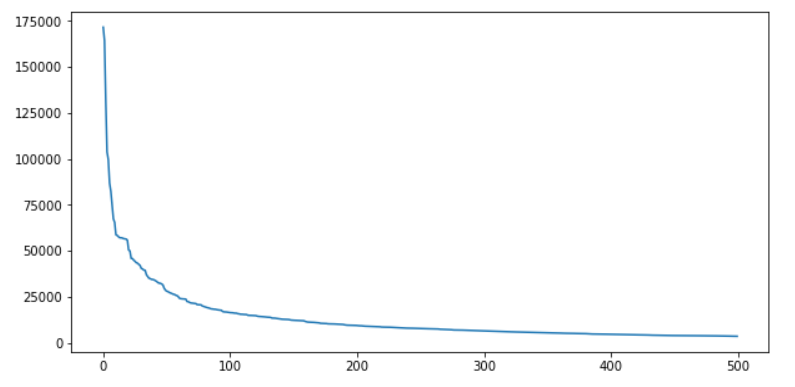
\includegraphics[scale=0.65]{Length.PNG}
  \caption{Frequency of the top 500 words}
\end{figure}
To create the dictionary out of the most frequently occurring words, we had to
start by tokenising each tweet. We used the tokens to count the occurrence of
every unique word, sort the words based on the frequency and only keep the top
25000 words. While counting the frequency of the tokens, we replace all twitter
user handles with the tag “<usr>”. We do this because naming another user in a
tweet can have a lot of meaning, but each user handle is unique, and they all
handles will be represented by a different token. We tried to negate this by
replacing all usernames with the same token. After creating the dictionary, we
replace every word with its index in the dictionary. If a word is not found, it
is replaced by a “<unk>” tag, which shows that the word is unknown. Now the
input data consist of arrays of varying sizes. The embedding layer requires all
input data to have the same shape. To decide the length of a tweet we did some
extra data analysis, we plotted the distribution of tweet lengths as seen in
figure 2.

\begin{figure}[H]
  \centering
  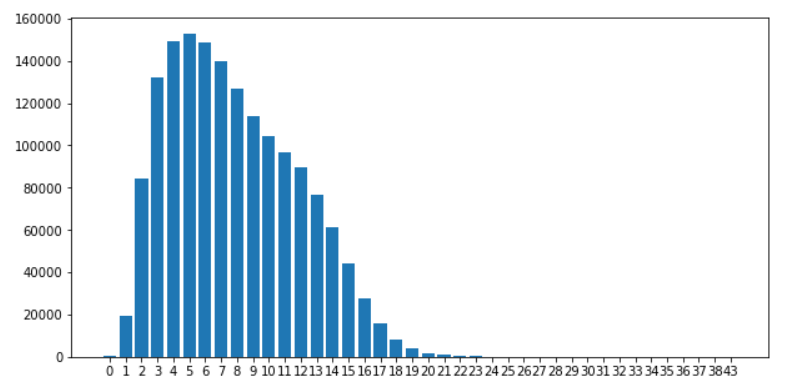
\includegraphics[scale=0.65]{Frequency.PNG}
  \caption{Distribution of the number of tokens tweets}
\end{figure}

The longest tweet has 43 tokens, but only one tweet has that many tokens. Most
tweets have between 1 and 20 tokens. We chose a length of 25 tokens, all tweets
with more than 25 tokens get reduced and all tweets with less than 25 tokens get
padded up to 25 tokens using “<pad>”. Now that the data is tokenised, padded and
transformed using a dictionary, we split it into training and test data using an
80\%-20\% split. Later while training the actual models, the training data is
split further into 80\% training and 20\% validation data .
\label{gen_inst}

The text must be confined within a rectangle 5.5~inches (33~picas) wide and
9~inches (54~picas) long. The left margin is 1.5~inch (9~picas).  Use 10~point
type with a vertical spacing (leading) of 11~points.  Times New Roman is the
preferred typeface throughout, and will be selected for you by default.
Paragraphs are separated by \nicefrac{1}{2}~line space (5.5 points), with no
indentation.

The paper title should be 17~point, initial caps/lower case, bold, centered
between two horizontal rules. The top rule should be 4~points thick and the
bottom rule should be 1~point thick. Allow \nicefrac{1}{4}~inch space above and
below the title to rules. All pages should start at 1~inch (6~picas) from the
top of the page.

For the final version, authors' names are set in boldface, and each name is
centered above the corresponding address. The lead author's name is to be listed
first (left-most), and the co-authors' names (if different address) are set to
follow. If there is only one co-author, list both author and co-author side by
side.

Please pay special attention to the instructions in Section \ref{others}
regarding figures, tables, acknowledgments, and references.

\section{Deep learning models}
\subsection{CNN}
We experimented using two different types of deep learning models. First, we
tried to train a Convolutional Neural Network (CNN). A CNN uses convolutional
layers, the main goal of the convolutional layer is to extract pattern or
specific features that occur often throughout the tweets in the training data.
This is combined with a pooling layer that aggregates the information gathered
from the previous layers and reduces the number of parameters [1]. A
representation of the architecture we used in our CNN can be seen in Figure 3.
\begin{figure}[H]
  \centering
  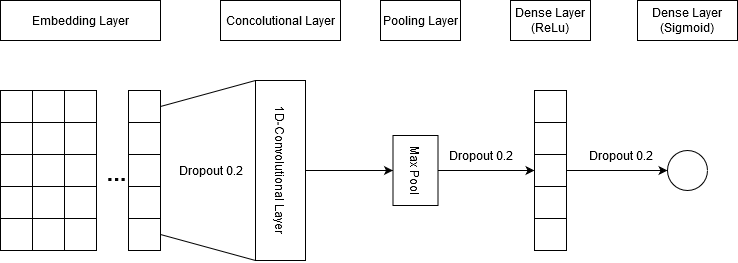
\includegraphics[scale=0.54]{CNN.png}
  \caption{CNN model}
\end{figure}
Our model starts with an embedding layer that trains word embeddings with 300
features. A one-dimensional convolutional layer with a kernel size of 3 and a
dimension size of 300. The results of the convolutional layer get pooled through
a Max Pooling layer with a pool size of 2. The results get flattened into a
one-dimensional array. The features extracted by the convolutional layer are
piped to a Dense layer with 150 nodes and finally to a Dense layer with one node
that makes the final prediction. To reduce overfitting, we have added a Dropout
of 0.2 after the embeddings and before each dense layer.
\subsection{RNN}
The other model is a Recurrent Neural Network (RNN) using long short-term memory
layers (LSTM). Unlike CNNs, when an RNN is trained using sequential data, the
internal weights are shared across the sequence [2]. A tweet is a sequence of
words, the LSTM layer looks at each word embedding in the sequence individually.
The input is not only a single word embedding, but it also receives an extra
input from the previous word. But sometimes there are words important to the
context that occur later in the sentence. This will have a small impact if the
LSTM only trains in one direction. That is why we used a Bidirectional LSTM,
this means that there is a layer that goes over the sequence normally and a
layer that goes over the sequence backwards. A representation of the
architecture we used in our RNN can be seen in Figure 3.
\begin{figure}[H]
  \centering
  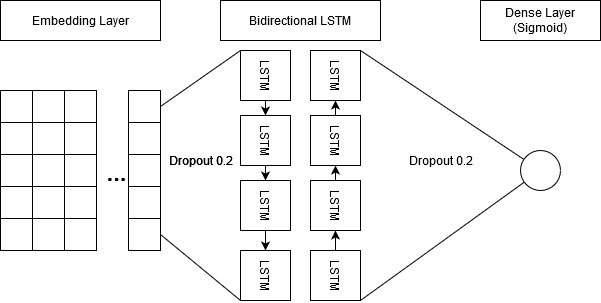
\includegraphics[scale=0.54]{RNN.png}
  \caption{RNN model}
\end{figure}
Our model starts with an embedding layer that trains word embeddings with 150
features. The word vectors are passed to a Bidirectional LSTM layer that has 80
nodes in each direction, making it a total of 160 nodes. Finally, the results of
the LSTM layer get passed to a Dense layer with 1 node and a sigmoid activation
layer to get the prediction. To reduce overfitting, we have added a dropout
layer of 0.2 after the embedding and before the dense layer.
\section{Experimentation}
We tried different variations for both neural networks. In both cases, we
trained multiple models with different configurations e.g. Features in the
embedding layer, more dense layers of varying sizes. That is how we found out
that an embedding layer with 150 features gives better results in the RNN while
the CNN model gave a better accuracy using an embedding layer with 300 features.

In the CNN we experimented with the dimension size and kernel size of the
convolutional layer. We trained the model using high and low values and chose to
use the configuration that gave us the best results. The first version of the
model did not have a hidden dense layer. But we found that adding it improves
the accuracy by 2\%. To choose the size of the hidden layer, we trained the
model \%using 50, 100, 150, 200 and 250 nodes and we found that a \%Dense layer with 150 nodes gave the best results.

We did the same thing with the LSTM layer in the RNN. Adding a hidden Dense
layer in this model made the model too complex and helped it overfit.

\subsection{Pre-trained word embeddings}
The RNN was the best out of the two models. We wanted to see if it was possible
to improve the model using pre-trained word embeddings. At the moment, the
embedding layer generated word vectors using our own data. Pre-trained word
embeddings are vectors that have been trained using a large dataset and are
saved so they can be reused in other NLP tasks. Examples of popular pre-trained
words embeddings are word2vec and GloVe These vectors are generated using bigger
datasets and more advanced methods than our embedding layer. We wanted to find
out if it would improve the accuracy of our models. We used the GloVe [3] word
vectors with 100 features, which was trained using Wikipedia dumps and Gigaword
corpora, by taking the embeddings of the words that appear in our dictionary and
using them to create an embedding matrix. The words that appear in both our
dictionary and the GloVe embeddings will have vectors, while the words that only
appear in our dictionary will have a vector of zeroes. The matrix then replaces
the weights of the embedding layer. We trained this model twice, first with a
disabled embedding layer so the vectors aren’t modified. Then with the weights
disabled so the embedding layer modifies the vectors based on our data.

\section{Results}

\section{Conclusions \& future work}


\small

[1] Severyn, A. and Moschitti, A., 2015, August. Twitter sentiment analysis with
deep convolutional neural networks. In Proceedings of the 38th International ACM
SIGIR Conference on Research and Development in Information Retrieval (pp.
959-962).

[2] Cliche, M., 2017. Bb\_twtr at semeval-2017 task 4: Twitter sentiment analysis with cnns and lstms. arXiv preprint arXiv:1704.06125.

\end{document}
